In this chapter, we evaluate the instrumentation for checking memory safety
that was employed in \symbiotic on benchmarks from SV-COMP 2018.

We used all the benchmarks from the official \emph{MemSafety} category along
with the benchmarks from the subcategory \emph{TerminCrafted} which was not
included in the official SV-COMP 2018. The benchmarks from these categories are
programs in C and they can contain either no violation of memory safety, or the
following errors:
\begin{itemize}
  \item invalid memory deallocation, e.g. double free error,
  \item invalid pointer dereference,
  \item memory leaks.
\end{itemize}
There were 390 benchmarks in total, 140 of them containing some
memory safety violation, 250 of them safe.


\symbiotic first instruments the program according to one of the configurations
described in Chapter~\ref{chap:memsafety}. Since the newly inserted code marks
possible error locations, we reduced the problem to a reachability problem.
\symbiotic slices the program and then runs symbolic executor \klee that checks
the reachability of the error locations. If no error location is reachable, it
answers \emph{true}. If some error location is reachable, it answeres
\emph{false} and gives information about a type of the error (e.g.  invalid
dereference or memory leak). If \symbiotic cannot decide the reachability, it
answers \emph{unknown}. If it runs out of time, i.e.~the given time limit
was exceeded, the answer is \emph{timeout}.

All the following measurements were taken on machines with \textit{Intel(R)
Core(TM) i7-3770} CPU that run on 3.40GHz frequency and dispose of 8~GB of
memory. The memory limit was set to 8~GB. We used the utility
\emph{Benchexec}~\cite{Beyer2015} for reliable measurement of consumed
resources.

\section{Comparison of Configurations}
In this section, we compare three configurations introduced in
Chapter~\ref{chap:memsafety}: the basic approach (one-phase instrumentation
without any plugins, denoted as \emph{basic}), the enhancement with a pointer
analysis as a plugin (denoted as \emph{ePTA}) and the staged instrumentation
(denoted as \emph{staged}). We ran \symbiotic with these configurations on the
above mentioned benchmarks with the CPU time limit set to 120~s.
\begin{table}[t]
\begin{tabular}{|p{6cm} || C{1.5cm} | C{1.5cm} | C{1.5cm}|}
 \hline
 & basic & ePTA & staged \\
 \hline
 \hline
 size before instrumentation & 155801 & 155801 & 155801 \\
 \hline
 size after instrumentation  & 322058 & 192496 & 171348 \\
 \hline
 inserted calls (total)    & 166257 & 36695 & 15547 \\
 \hline
 inserted calls (average)  & 426 & 94 & 39 \\
 \hline
\end{tabular}
\caption{The comparison of the three configurations for the memory safety
instrumentation. Size is given by the number of instructions of a program.}
\label{tab:numbers}

\end{table}

As for the number of inserted instructions, we present the experimental results
in Table~\ref{tab:numbers}. The first part of the table shows the total size of
the benchmarks expressed with the number of LLVM instructions before and after
instrumentation for each configuration. In the second part, the cumulative and
average number of inserted \texttt{call} instructions is counted. Note that the
total size before instrumentation is 155801 instructions, which is 400
instruction on average. This means that with the basic approach, the final code
after instrumentation is of more than double size. Evidently, the number of
inserted instructions significantly decreases with each enhancement.  This is
also depicted in Figure~\ref{fig:increase_chart} that shows the increase of the
total number of instructions expressed in percentage.

\begin{figure}[h]
  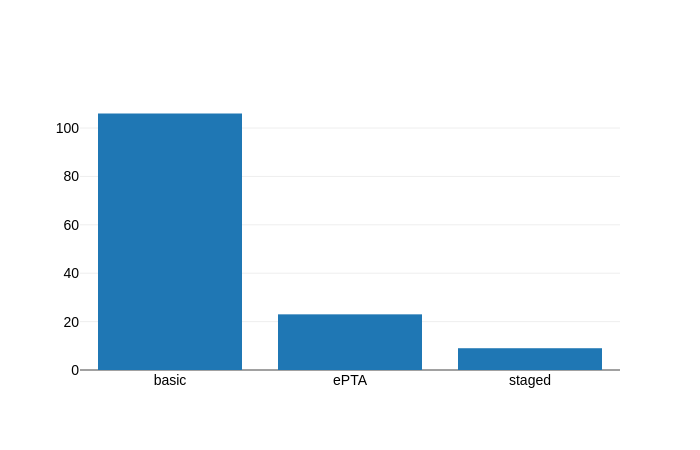
\includegraphics[width=\textwidth]{charts/bar_chart.png}
  \caption{The total increase of the number of instructions in \% when using
  the three configurations for the memory safety instrumentation.}
  \label{fig:increase_chart}
\end{figure}

\todo{times}

\begin{table}[t]
\begin{tabular}{|l || r | r | r|}
 \hline
 & basic & ePTA & staged \\
 \hline
 \hline
 true     & 116 & 123  & 183 \\
 \hline
 false    & 132 & 133  & 135 \\
 \hline
 timeout  & 139 & 130  & 71 \\
 \hline
\end{tabular}
\caption{The numbers of \emph{true}, \emph{false} and \emph{timeout} answers
given by \symbiotic when using the three configurations for the memory safety
instrumentation.}
\label{tab:answers}

\end{table}

The reduced number of inserted instruction had indeed a positive effect on the
answers of \symbiotic as shown in Table~\ref{tab:answers}. When using the basic
approach, \symbiotic did not manage to decide 139 benchmarks in the given time
limit. With a pointer analysis, the number of timeouts slightly decreased. The
most significant improvement was achieved with the staged instrumentation:
\symbiotic ran out of time only in 71 cases. The both enhancements had impact
especially on the benchmarks that did not contain any violation of memory
safety.

